\begin{frame}
	\frametitle{\contentsname}

	\tableofcontents
	\begin{picture}(0,0)
		\put(420,200){\makebox(0,0)[rt]{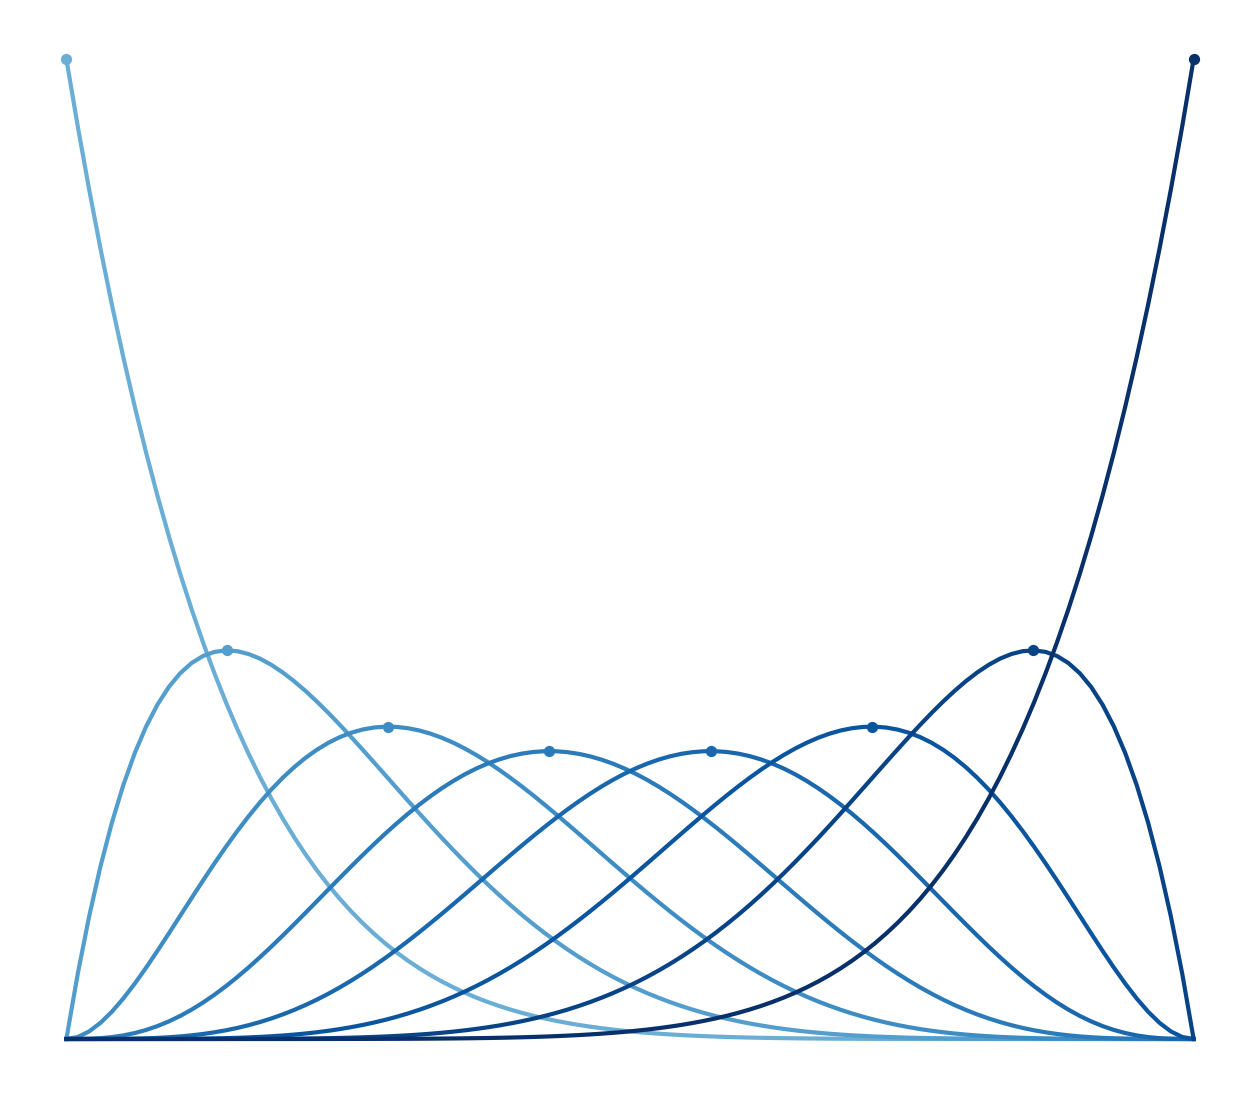
\includegraphics[width=0.5\paperwidth]{bernstein}}}
	\end{picture}

	\note{
		The talk is divided in five sections.

		\

		\begin{enumerate}
			\item

			      We will show the objectives.

			\item

			      We will show a lot of definitions.

			\item

			      We will develop lemmas and the proof of approximation theorem.

			\item

			      In the fourth one, we will stablish the title's theorem.

			\item

			      In the fifth one, we will show some theoretical applications and simulations.
			      For example, the universal approximation.
		\end{enumerate}

		\

		Feel free to ask anytime.

		\

		Let's start!
	}
\end{frame}